\chapter{Black hole formation 2: Vaidya collapse}
\label{s:vai}

\minitoc

\section{Introduction}

Having investigated the gravitational collapse of a star, modeled as a ball of dust,
in the preceding chapter, we turn now to a less astrophysical scenario: the
formation of a black hole by the collapse of a shell of radiation,
known as \emph{Vaidya collapse}. Albeit quite
academic, this process illustrates various features of black hole birth and dynamics.

\section{The ingoing Vaidya metric}

\subsection{General expression} \label{s:vai:general}

Let us consider a spherically symmetric spacetime $(\M,\w{g})$ described by
coordinates $(v,r,\th,\ph)$ such that $v\in \R$, $r\in(0, +\infty)$,
$\th\in(0,\pi)$ and $\ph\in(0,2\pi)$, $(\th,\ph)$ being standard
spherical coordinates on $\SS^2$ and $r$ being the areal radius associated
with spherical symmetry (cf. Sec.~\ref{s:sch:static_spher}).
The \defin{ingoing Vaidya metric}\index{ingoing!Vaidya metric}\index{Vaidya!metric!ingoing --}
is the metric tensor
\be \label{e:vai:Vaidya_metric_null}
    \encadre{ \w{g} =
            -\left( 1 - \frac{2 M(v)}{r} \right)\, \dd v^2
            + 2 \, \dd v \, \dd r
        + r^2 \left( \dd\th^2 + \sin^2\th\, \dd\ph^2 \right) } ,
\ee
where $M(v)$ is a real-valued function of $v$.
We immediately notice that this expression strongly resembles that
of the Schwarzschild metric expressed in the
\emph{null ingoing Eddington-Finkelstein}\index{Eddington-Finkelstein!coordinates}\index{null!ingoing Eddington-Finkelstein coordinates}
coordinates, as given by Eq.~(\ref{e:sch:Schwarz_metric_NIEF}). Actually, the
only difference is the constant $m$ in Eq.~(\ref{e:sch:Schwarz_metric_NIEF})
replaced by the function $M(v)$ in Eq.~(\ref{e:vai:Vaidya_metric_null}).
We may say that the Schwarzschild metric is the special case $M(v) = m$ of
the ingoing Vaidya metric.

A key property of the ingoing Vaidya metric is
\begin{greybox}
The vector field $\w{k}$, defined as the metric-dual\footnote{Cf. Sec.~\ref{s:bas:metric_dual};
in index notation: $k^\alpha := - g^{\alpha\mu} \partial_\mu v = - \nabla^\alpha v \iff
k_\alpha := - \partial_\alpha v $}
of the 1-form $-\dd v$:
\be \label{e:vai:def_k}
    \w{k} := - \vp{\dd v} = - \vw{\nabla} v \quad\iff\quad
    \uu{k} := - \dd v ,
\ee
is a null vector.
\end{greybox}
\begin{proof}
In view of the metric components (\ref{e:vai:Vaidya_metric_null}),
the coordinate vector field $\wpar_r$ is a null vector, since $g_{rr} = 0$.
Its metric-dual is the 1-form
$\uu{\wpar_r} = g_{\mu r}\dd x^\mu = g_{vr} \dd v = \dd v = - \uu{k}$.
Hence
\be \label{e:vai:k_d_dr}
    \w{k} = - \left. \der{}{r} \right| _{v,\th,\ph} ,
\ee
where we have rewritten the null vector $\wpar_r$ as $\left. \dert{}{r} \right| _{v,\th,\ph}$
to distinguish it from the vector $\wpar_r$ of the IEF coordinates, to be
introduced in Sec.~\ref{s:vai:IEF}. It follows that $\w{k}$ is a null vector.
\end{proof}

Since $\dd v$ is nowhere vanishing, $\w{k}$ is a nonzero null vector field on $\M$.
We may use it to set up the \emph{time orientation} of $(\M,\w{g})$
by declaring that $\w{k}$ is future-oriented (cf. Sec.~\ref{s:fra:time_orientation}).

As shown in the notebook~\ref{s:sam:Vaidya},
the Ricci tensor of $\w{g}$ is very simple:
\be
    \w{R} = \frac{2 M'(v)}{r^2}\, \dd v \otimes \dd v ,
\ee
where $M'(v)$ stands for the derivative of the function $M(v)$.
The Ricci scalar $R = g^{\mu\nu} R_{\mu\nu} = (2M'(v)/r^2) \, \nabla_\mu v \nabla^\mu v =  (2M'(v)/r^2) \, k_\mu k^\mu$ is identically zero, since $\w{k}$ is a null vector.
It follows that
\begin{greybox}
The ingoing Vaidya metric (\ref{e:vai:Vaidya_metric_null}) is a solution
of the Einstein equation (\ref{e:fra:Einstein_eq})
with $\Lambda = 0$ and with the energy-momentum tensor
\be \label{e:vai:ener_mom_tensor}
   \encadre{ \w{T} = \frac{M'(v)}{4\pi r^2}\, \uu{k} \otimes \uu{k}  } .
\ee
\end{greybox}
The tensor (\ref{e:vai:ener_mom_tensor}) has the same
structure as the energy-momentum tensor of the dust model considered in Chap.~\ref{s:lem}:
$\w{T}_{\rm dust} = \rho  \, \uu{u} \otimes \uu{u} $ [Eq.~(\ref{e:lem:T_pressureless})].
The main difference is that $\w{u}$ is a timelike vector (the dust 4-velocity), while
$\w{k}$ is a null vector. For this reason, the energy-momentum tensor  (\ref{e:vai:ener_mom_tensor})
is sometimes referred to as a \defin{null dust}\index{null!dust}\index{dust!null --} model \cite{Poiss04}.
It corresponds physically to the energy-momentum tensor of some \emph{electromagnetic radiation} in the
\emph{geometrical optics}\index{geometrical optics} approximation (see Box~22.4 of Ref.~\cite{MisneTW73}):
$\w{T}_{\rm rad} = q  \, \uu{K} \otimes \uu{K}$, where $q\geq 0$ and $\w{K} := \vw{\nabla}\Phi$ is the \emph{wave vector}\index{wave!vector}, $\Phi$ being the rapidly-varying
phase in the geometrical optics decomposition $\w{A} = \mathrm{Re}(\mathrm{e}^{\mathrm{i}\Phi} \, \w{a})$ of the electromagnetic potential 1-form $\w{A}$. The quantity $q$ is related to the energy density
$\veps$ of the electromagnetic field as measured by an observer $\Obs$ of 4-velocity $\w{u}$
by $\veps = \omega^2 q$, where $\omega = - \w{K}\cdot\w{u}$ is the frequency of the electromagnetic
radiation as measured by $\Obs$.
Maxwell equations\index{Maxwell equations} imply that $\w{K}$ is a null vector and that it is geodesic:
$\w{\nabla}_{\w{K}}\, \w{K} = 0$. The geodesic field lines of $\w{K}$ are nothing but
the \emph{light rays}\index{light!ray} of the geometrical optics framework.
The geodesic character also holds for $\w{k}$ as defined by Eq.~(\ref{e:vai:def_k})
(cf. the notebook~\ref{s:sam:Vaidya} for an explicit check):
\be \label{e:vai:k_geodesic}
    \w{\nabla}_{\w{k}}\, \w{k} = 0 .
\ee
It follows then from the identity (\ref{e:vai:k_d_dr}) that the curves $(v,\th,\ph) = \mathrm{const}$
are null geodesics, $\lambda:=-r$ is an affine parameter along them and $\w{k}$ is
the corresponding tangent vector.

Another condition for the identification of $\w{T}$ with $\w{T}_{\rm rad}$ is that the coefficient
in front of $\uu{k} \otimes \uu{k}$ in (\ref{e:vai:ener_mom_tensor})
is non-negative, since $q\geq 0$ in $\w{T}_{\rm rad}$. This constraint can also be seen as the \emph{null energy condition} (\ref{e:neh:null_energy_cond}) introduced in
Sec.~\ref{s:neh:NEH_Theta_zero}: for any null vector $\wl$, we have
$\w{T}(\wl,\wl) = M'(v)/(4\pi r^2)\, (\w{k}\cdot\wl)^2$ and hence $\w{T}(\wl,\wl) \geq 0$ $\iff$
$M'(v) \geq 0$. In other words, the function $M(v)$ must be monotically increasing. Then, we can set
$\w{k} = \alpha \w{K}$, where $\alpha$ is a constant, to have a perfect match of (\ref{e:vai:ener_mom_tensor}) with the electromagnetic radiation energy-momentum
tensor $\w{T}_{\rm rad}$.
To summarize:
\begin{greybox}
Provided that $M(v)$ is an increasing function\footnote{by \emph{increasing}, it is meant
strictly increasing ($M'(v)>0$) or locally constant ($M'(v) = 0$).},
the ingoing Vaidya spacetime $(\M,\w{g})$ is generated by a spherical symmetric electromagnetic radiation
within the geometrical optics approximation. The corresponding light rays are the
ingoing radial null geodesics
defined by $v=\mathrm{const}$, $\th=\mathrm{const}$ and $\ph=\mathrm{const}$.
These geodesics admit $\w{k}$ as the tangent vector associated with their affine parameter
$\lambda := -r$.
\end{greybox}

\subsection{Expression in ingoing Eddington-Finkelstein coordinates} \label{s:vai:IEF}

To deal with the black hole formation in Vaidya spacetime, it will quite
convenient to work with the
\defin{ingoing Eddington-Finkelstein (IEF) coordinates}\index{Eddington-Finkelstein!coordinates}\index{ingoing!Eddington-Finkelstein!coordinates}\index{IEF}
$(t,r,\th,\ph)$ defined from the null coordinates $(v,r,\th,\ph)$ in the
same way as for the Schwarzschild case, i.e. such that $v$ is the
\defin{advanced time}\index{advanced!time}\index{time!advanced --} with respect to $t$
[cf. Eq.~(\ref{e:sch:ti_v_r})]:
\be  \label{e:vai:t_v_r}
    \encadre{t := v - r} \iff \encadre{v = t + r} .
\ee
\begin{remark}
The coordinate $t$ was denoted by $\ti$ in Chap.~\ref{s:sch}, where $t$
was reserved for the Schwarzschild-Droste time coordinate.
\end{remark}
We have $\dd v = \dd t + \dd r$, from which the IEF expression of the
metric tensor is immediately deduced from Eq.~(\ref{e:vai:Vaidya_metric_null}):
\be \label{e:vai:metric_IEF}
    \encadre{
        \begin{array}{ll}
        \w{g} = &
           \displaystyle -\left( 1 - \frac{2 M(t+ r)}{r} \right)\, \dd t^2
            + \frac{4 M(t + r)}{r} \, \dd t \, \dd r
            + \left( 1 + \frac{2 M(t+r)}{r} \right)\, \dd r^2 \\[1ex]
       & + r^2 \left( \dd\th^2 + \sin^2\th\, \dd\ph^2 \right) .
       \end{array}
       }
\ee
The expression of $\w{k}$ in terms of the IEF coordinate frame
is deduced from Eq.~(\ref{e:vai:k_d_dr}) and the chain rule:
\be
    \w{k} = \wpar_t - \wpar_r .
\ee
\begin{remark}
The analog equation in Schwarzschild spacetime is Eq.~(\ref{e:sch:null_vector_k}).
\end{remark}

\begin{figure}
\centerline{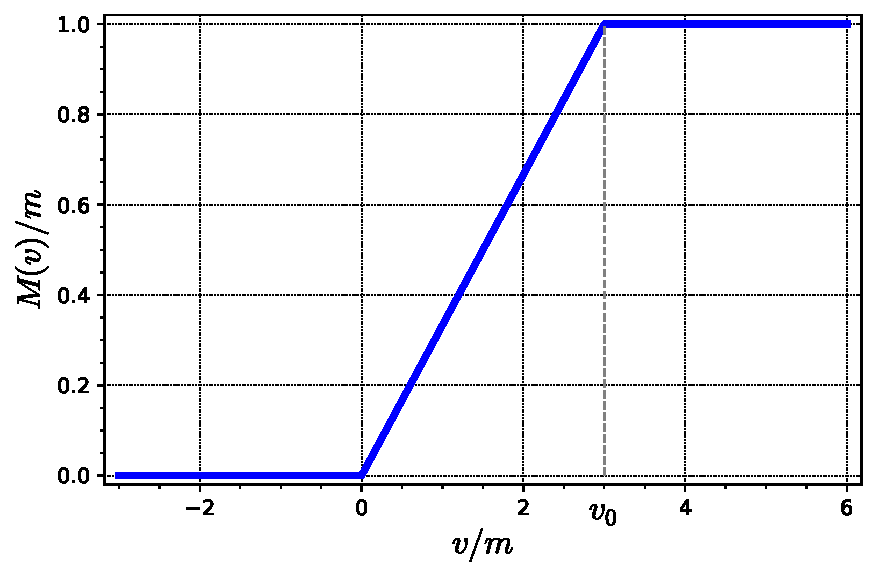
\includegraphics[width=0.6\textwidth]{vai_mass_function.pdf}}
\caption[]{\label{f:vai:mass_function} \footnotesize
An example of function $M(v)$ increasing linearly on $[0,v_0]$.
}
\end{figure}




\subsection{Case of an infalling shell of radiation}

An \defin{infalling shell of radiation}\index{shell!infalling -- of radiation}\index{infalling!shell of radiation}
is defined by the function $M(v)$ obeying
$M'(v) \neq 0$ only on a finite interval of $v$. By choosing properly
the origin of $v$, we may consider this interval to be $[0, v_0]$, with
the parameter $v_0>0$ governing the
thickness of the shell.
The function $M(v)$ is thus constant outside the interval $[0, v_0]$.
In order to describe the formation of a black hole, we choose
$M(v) = 0$ for $v < 0$. This corresponds to a piece of Minkowski spacetime,
since the metric (\ref{e:vai:metric_IEF})
cleary reduces to Minkowski metric wherever $M(v)=0$ [compare Eq.~(\ref{e:glo:Mink_metric_spher})].
Denoting by $m>0$ the constant value of $M(v)$ for $v > v_0$, we have then
\be \label{e:vai:mass_function}
    M(v) = \left\{ \begin{array}{ll}
     0 \quad \mbox{for} \ v < 0 \qquad & \mbox{(Minkowski region)} \\
     \mbox{increases from}\ 0 \ \mbox{to}\ m \quad \mbox{for} \ 0 \leq v \leq v_0
        & \mbox{(radiation region)} \\
      m \quad \mbox{for} \ v > v_0 \qquad & \mbox{(Schwarzschild region).}
      \end{array} \right.
\ee
The region for $v>v_0$ is denoted \emph{Schwarzschild} since for $M(v) = m = \mathrm{const}$,
the Vaidya metric reduces to Schwarzschild metric, as we have already noticed
in Sec.~\ref{s:vai:general}. The simplest example of a function $M(v)$
obeying (\ref{e:vai:mass_function}) is $M(v) = m v/v_0$ for $v\in[0, v_0]$;
it is shown in Fig.~\ref{f:vai:mass_function} for $v_0 = 3 m$.

\subsection{Black hole formation}

%%%%%%%%%%%%%%%%%%%%%%%%%%%%%%%%%%%%%%%%%%%%%%%%%%%%%%%%%%%%%%%%%%%%%%%%%%%%%%%

\section{Trapping horizon}















